\chapter[SAX-P]{Symbolic representation of cyclic time series based on properties of cycles}
\label{chapter_saxp}
%\minitoc

\begin{abstract} 
The analysis of cyclic time series from bio-mechanics is based on the
comparison of the properties of their cycles. As usual algorithms of time 
series classification ignore this particularity, we propose
a symbolic representation of cyclic time series based on the properties
of cycles, named SAX-P. The resulting character strings can be compared
using the Dynamic Time Warping distance. The application of SAX-P
to propulsive moments of three subjects (S1, S2, S3) moving in Manual
Wheelchair highlight the asymmetry of their propulsion. The symbolic representation SAX-P facilitates the reading of the cyclic time series and the clinical interpretation of the classification results.
\end{abstract} 

\section{Introduction}
\label{introduction}

Generally, during his locomotion, the human being performs cyclic movements (e.g. : walking, running, swimming,
cycling). The bio-mechanical analysis of these movements is performed with various measuring instruments 
(eg force and acceleration sensors, kinematic analysis systems) that enable continuous recording over 
long periods of many kinematic and dynamic parameters. These recordings produce long
time series composed of many cycles or patterns, representative of the movements made and effort 
produced by the subject during his displacement (Fig. \ref{fig:cyclicTS}).


 \begin{figure}[h]
  \centering
   \includegraphics[scale=0.4]{images/sax-p/cycliqueTS}
    \caption{Cyclic time series form manual wheelchair locomotion}
  \label{fig:cyclicTS}
  \end{figure}


These cycles are the time series analysis units and have several
characteristic properties such as the minimum value, the area under the cycle 
\cite{Vegter2014} (Fig. \ref{fig:cycleProp}). 

 \begin{figure}[h]
  \centering
   \includegraphics[scale=0.4]{images/sax-p/cycle_prop}
    \caption{Properties of a cycle}
  \label{fig:cycleProp}
  \end{figure}
	

For comparing time series, several previous studies suggested to break them into 
small segments and then to compare the properties of their segments.
A segment of a time series is a sequence of consecutive values belonging to it \cite{Abonyi2003}.


\cite{keogh2001dimensionality} proposed replacing each segment of a time series
$X=x_{1},x_{2},\cdots,x_{n}$ by its mean values;
$\bar{x}_{i}=\frac{N}{n}\sum_{j=\frac{n}{N}(i-1)+1}^{(\frac{n}{N})i}x_{j},$  transforming the time
series, which is a sequence of values, in the suite of the means of its N segments
$\bar{X}=\bar{x}_{1}\bar{,x}_{2},\cdots,\bar{x}_{N}.$ This method is known as Piecewise Aggregate
Approximation (PAA) (Fig. \ref{fig:paa}). The time series $C$ and $Q$ are then compared by calculating the distance $DR$
between the suite $\bar{C}$ and $\bar{Q}$ of the means of their segments :
\begin{equation}
DR(\bar{C},\bar{Q})=\sqrt{\frac{n}{N}\sum_{i=1}^{N}(\bar{c}_{i}-\bar{q}_{i})^{2}}.
\label{equ:paa}
\end{equation}

 \begin{figure}[h]
  \centering
   \includegraphics[scale=0.4]{images/sax-p/paa}
    \caption{Piecewise aggregate approximation of a cyclic time series}
  \label{fig:paa}
  \end{figure}

The main objective of PAA was to reduce the length of the time series. However, 
as it computes the segments means, it also allows us to compare two time series C and Q from 
the properties of their 
segments (Equation \ref{equ:paa} ).


\cite{lin2003symbolic} were based on the PAA method to provide a symbolic representation of time
series called Symbolic Aggregate Approximation (SAX). The objective of SAX is to assign a letter to
each segment. To do this, the domain of the values of the time series is divided into intervals
so that every point of the temporal series has approximately the same probability to belong to an 
interval and a letter is associated with each of these intervals.  Then each segment of the time
series is associated with the letter of the interval  to which belongs its average (Fig. \ref{fig:sax}).

 \begin{figure}[h]
  \centering
   \includegraphics[scale=0.6]{images/sax-p/sax2}
    \caption{Symbolic Aggregate approXimation of a cyclic time series}
  \label{fig:sax}
  \end{figure}
	

With SAX, the distance $MINDIST$ between two strings $\hat{Q}$ and $\hat{C}$ of length $N$ is calculated from the
distance between the borders of the intervals represented by each character in the string 
(Equation \ref{equ:sax}).


\begin{equation}
MINDIST(\hat{Q},\hat{C})=\sqrt{\frac{n}{N}\sum_{i=1}^{N}(dist(\hat{q}_{i},\hat{c}_{i}))^{2}}.
\label{equ:sax}
\end{equation}


$\hat{q}_{i}\:et\:\hat{c}_{i}$ are characters and $ dist() $ is the distance between the borders of 
the intervals which represent these characters  \cite{lin2003symbolic}. However, two segments with very 
different shapes can have the same average and be represented by the same letter: the mean is not 
enough to define a segment. In order to solve this problem, \cite{Lkhagva2006} proposed the ESAX 
model that considers three properties for each segment: its mean, its minimum and maximum (Fig. \ref{fig:esax}).

 \begin{figure}[h]
  \centering
   \includegraphics[scale=0.6]{images/sax-p/Esax}
    \caption{Extended Symbolic Aggregate approXimation of a cyclic time series}
  \label{fig:esax}
  \end{figure}

Thereafter, \cite{sun2014improvement} proposed the SAX-TD model that takes into account 
 two properties for each segment: its mean and trend. They then adjust the distance used by the SAX 
 method for it to take into account the trend (Fig. \ref{fig:saxtd}).

 \begin{figure}[h]
  \centering
   \includegraphics[scale=0.4]{images/sax-p/Sax-td}
    \caption{Trend Symbolic Aggregate approXimation of a cyclic time series}
  \label{fig:saxtd}
  \end{figure}
	
	 \begin{figure}[h]
  \centering
   \includegraphics[scale=0.4]{images/sax-p/unD_sax}
    \caption{Properties of a cycle}
  \label{fig:1dsax}
  \end{figure}

Both methods provide better results than the SAX method \cite{sun2014improvement}. However, they have the
disadvantage of increasing the number of symbols required to represent the time series. Indeed, 
the method ESAX triple the size of the representation of a time series provided by the SAX method, 
while the SAX-TD method the double. In addition,  the previous four methods have two major drawbacks: 
they consider fixed-size segments, while the cycles are variable-sized segments, and they do not take into account the characteristic properties of cycles such as 
the duration and the surface under a cycle. Our goal is to provide a symbolic representation that 
takes into account several properties for each cycle, but without increasing the number of symbols 
used for the representation.


 The symbolic representations obtained have another advantage;
they allow to use a large number algorithms available
for sequence analysis like novelty detection (finding
unusual shapes or sub-sequences), motif discovery (finding
repeated shapes or sub-sequences) \cite{Begum2014}, clustering, classification,
indexing and also some interesting algorithms for
text processing or the bio-informatics community \cite{Aach2001, Papapetrou2011, Dietterich2002}. 

\section{SAX-P}

A prerequisite to be able to build a symbolic representation based on the cycles of the cyclic time series is to be able to segment the cyclic time series into consecutive cycles.

\subsection{Segmentation of cyclic time series}
The principle used to segment cyclic time series is as follows: A cycle contains all the data points between the beginning of two consecutive peaks. To locate the peaks, we set a threshold (Fig. \ref{fig:seuil}). The threshold considered can be the first or the second quartile of the time series data point.

	 \begin{figure}[h]
  \centering
   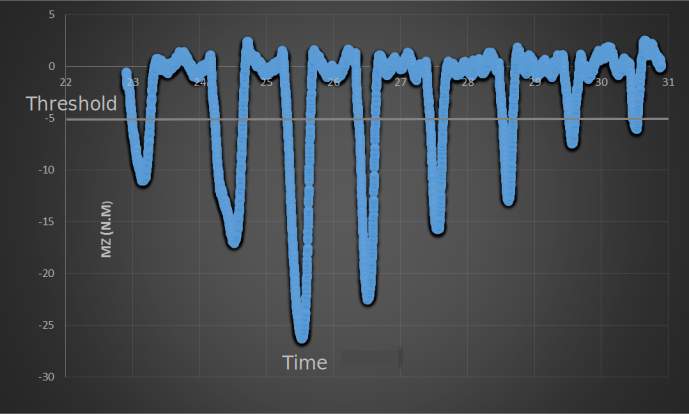
\includegraphics[scale=0.4]{images/sax-p/sax-p_deplacement_seuil}
    \caption{Threshold for the segmentation of cyclic time series}
  \label{fig:seuil}
  \end{figure}

If the current value of the time series is below this threshold, then it is a peak. It is then necessary to turn back to find the moment of the beginning of the peak. The figure (Fig. \ref{fig:segmentation}) presents the results obtained after segmentation of a cyclic time series.

	 \begin{figure}[h]
  \centering
   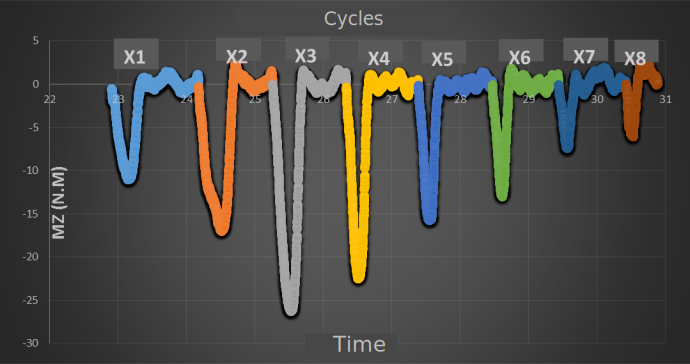
\includegraphics[scale=0.4]{images/sax-p/sax-p_deplacement32_thesee}
    \caption{Segmentation}
  \label{fig:segmentation}
  \end{figure}
	
\subsection{From cycles to letters}
The method SAX-P is based on SAX and works as follows:  
\begin{enumerate}
\item A cyclic time series is split in successive segments using a threshold
for identifying the beginning and the end of cycles, which have variable
durations;	
\item Several parameters (properties) are computed on each segment: cycle
time, push time, mean, median, standard deviation, minimum and maximum
values, and the area under the time series curve. As all these parameters
have different units, they must be normalized (i.e. centered and reduced) (Fig. \ref{fig:property} );

	 \begin{figure}[h]
  \centering
   \includegraphics[scale=0.4]{images/sax-p/sax-p_deplacement_property}
    \caption{Some properties are computed on each cycle}
  \label{fig:property}
  \end{figure}
	
 
\item Segments are then gathered in clusters using a classification algorithm \\
\cite{Esling2012} and each cluster is named by a capital letter (Fig. \ref{fig:classification}); 

	 \begin{figure}[h]
  \centering
   \includegraphics[scale=0.4]{images/sax-p/regroupement}
    \caption{Classification of cycles based on properties}
  \label{fig:classification}
  \end{figure}
	
	
\item Each segment is replaced by the letter of the cluster to which it
belongs, so that the initial cyclic time series is then represented
by a string of characters (Fig. \ref{fig:symbolic}); 

	 \begin{figure}[h]
  \centering
   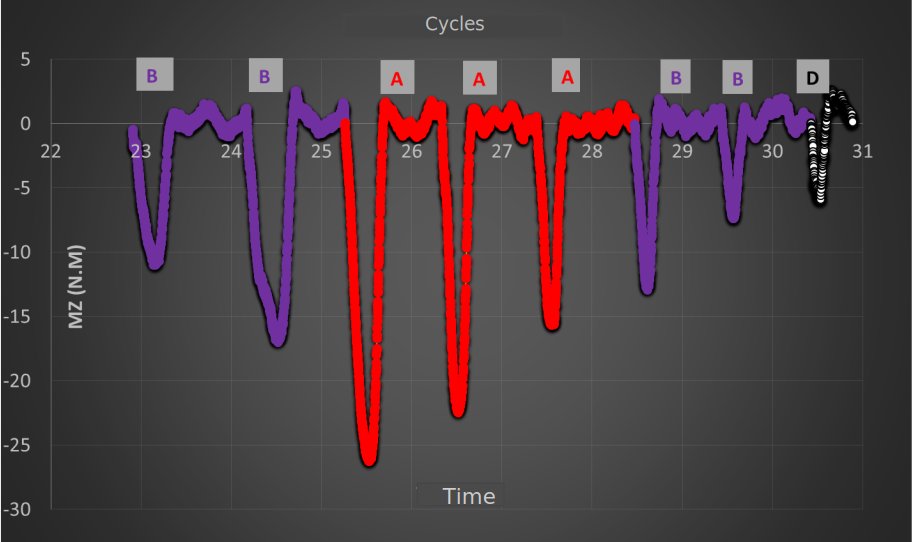
\includegraphics[scale=0.4]{images/sax-p/representionSymbolique2_t}
    \caption{Symbolic representation of cyclic time series}
  \label{fig:symbolic}
  \end{figure}
	
 \end{enumerate}

The distance between two strings, which may have different numbers
of characters, is computed using Dynamic Time Warping \cite{Petitjean2014} which is known as the
best distance measure for several domains \cite{Ding2008}. The distance between two characters is
the euclidean distance between the centers of the classes represented by those characters.

Unlike SAX, ESAX and SAX-TD methods that require  to fix the length of segments to consider when 
building the symbolic representation of a time series, SAX-P considers the cycles which
constitute basic unit of analysis of time series recorded during cyclic movements and also 
allows taking into account several characteristic features for each cycle. Figure \ref{fig:symbolic}
presents the symbolic representations obtained with the SAX method (in small letters) and SAX-P (in
capital letters). It illustrates that SAX-P unlike SAX considers cycles of the time series during
the construction of the symbolic representation.

%\begin{figure}[ht]
%\vskip 0.2in
%\begin{center}
%\centerline{\includegraphics[width=\columnwidth]{methode.png}}
%\caption{A cyclic time series is segmented in 5 propulsion cycles  
%(X1, X2, X3, X4, X5). For each cycle, a set of properties was 
%calculated and cycles with similar properties are gathered in 
%the same class (A or B). The original time series is thus transformed 
%into a string (here: AAABB).}
%\label{fig:methode}
%\end{center}
%\vskip -0.2in
%\end{figure} 

%\begin{figure}[ht]
%\vskip 0.2in
%\begin{center}
%\centerline{\includegraphics[width=\columnwidth]{representationS2.png}}
%\caption{Example of cyclic time series: propulsive moment applied by
% the subject S1  to the rear wheel of a Manual Wheelchair for a rectilinear
%  movement. Vertical bars delimit the propulsion cycles (segments) 
%  identified during this run, and the capital letter above each 
%  cycle indicates the cluster to which it belongs. Applying SAX to the propulsive moment divide
%  the time series into 10 segments of equal size (lowercase letter) regardless of propulsion cycles.
%  The area under the cycle, the cycle time and the pushed time are not taken into account by SAX.}
%\label{fig:moment}
%\end{center}
%\vskip -0.2in
%\end{figure} 

\section{Application to manual wheelchair locomotion}
\subsection{Dataset description}
The data sets used throughout these tests have been obtained from experiments  conducted with 12 subjects\footnote{The measurements made with subject S01 being of very low intensity, they were not considered during our analysis.} with disabilities in the aim to understand MWC locomotion. The measurements produced cyclic, uncertain and noisy time series (Fig. \ref{TWMWC}). All subsequent processing and analyses are performed on z-moment time series measured on both rear wheels of the FRET-2.

\begin{figure}[h]
\center
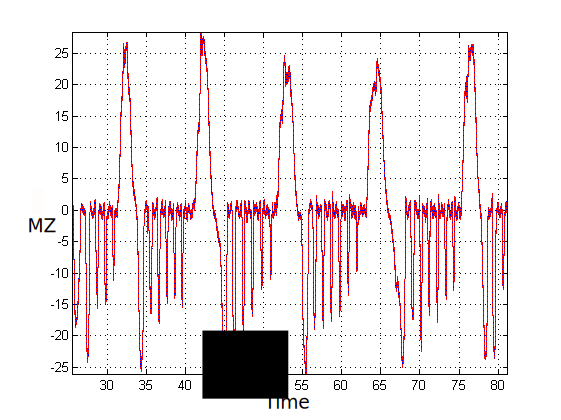
\includegraphics[scale = 0.5]{images/TSMWC}
\caption{Example of a z-moment (Mz) time series measured on the [left/right] rear wheel of the FRET-2.}
\label{TWMWC}
\end{figure}

The data recorded have four main characteristics:
\\
\textbf{Length of time series:} the length of the time series is due to the high acquisition frequency (100 Hz) of the force and torque sensor. For instance, a 10-minute recording generates a time series of:

\[
100 \, Hz \times 60 \, s \times 10 mn = 60,000 \, data \,points.
\]

The maximum length ($107,227$ data points) of the time series analysed here was reached by the z-moment of the left wheel of subject S02 (Fig. \ref{TWMWC}). The length of time series is a crucial issue because their processing time is highly dependent on their length. As an illustration, the time complexity of comparing two time series using the DTW alignment algorithm is $O(n^2)$ where $n$ is the length of the time series.
\\
\textbf{Cycles in time series:} The cyclic aspect of the time series comes from the cyclic nature of wheelchair propulsion. Indeed, this movement consists in a succession of push periods during which the user applies a force on the handrim of the wheelchair to propel it, and free-wheel periods during which the user moves his trunk and arms backwards for preparing the next push. The push phase is recorded by the sensor and materialized by a peak in Mz measurements, whereas during freewheel periods Mz values are close to zero (Fig. \ref{noisyTS}).

\begin{figure}[h]
\center
\includegraphics[scale = 0.5]{images/TSN}
\caption{Time series recorded by torsor sensor are noisy}
\label{noisyTS}
\end{figure}

\paragraph{}\textbf{Uncertainty in time series:} The presence of uncertainty in sensor measurements is intrinsic to the calibration process of sensors in general, and of the six-component dynamometer used in this work. When a force is applied to a piezo-resistive sensor, it causes a deformation of the sensing element, which consists in strain gauges \footnote{https://fr.wikipedia.org/wiki/Jauge\_de\_d\%C3\%A9formation} stuck on a small metallic beam and connected as a Wheatstone bridge \footnote{https://fr.wikipedia.org/wiki/Pont\_de\_Wheatstone} This deformation induces a change in the resistance of the strain gauges and thus a change in the output voltage of the Wheatstone bridge. According to Hooke's law, this is proportional to the force intensity. Thus, when using a calibrated sensor, the user is to measure a variation in sensor signal and uses the proportionality relationship (Hooke's law) to infer the intensity of the force that has been applied. Calibrating a sensor consists in constructing this proportionality relationship by applying a wide range of forces on the sensor, within the limits of the mechanical characteristics of the sensing element. Doing so, we record a sequence of couples of force intensity and electrical voltage, which is used to compute a regression line which will then be used to deduce the applied force intensity knowing the voltage variation. However, the regression line generally does not define a perfect proportionality relationship; in fact, it minimizes the error made but does not cancel it. This error (Fig. \ref{residus}) introduces uncertainty into the estimation of the applied force intensity. It is thus essential to take this error into account when evaluating time series to extract relevant information from them. Characterization of uncertainty is a time-consuming task (Appendix \ref{pdf_uncertainty}) and is not always possible because sensor calibration data are generally not available. 

\begin{figure}[h]
\center
\includegraphics[scale = 0.5]{images/residus}
\caption{Plot of Mz residues, which represent the differences between
Mz values measured by the sensor and real values applied during the calibration process.}
\label{residus}
\end{figure}

\paragraph{}\textbf{Noise in time series:} n the time series analysed here, the noise comes from the sensitivity of the dynamometer, which has been designed to measure low-intensity forces applied to the handrim during wheelchair locomotion. These forces can come from the texture of the ground (e.g. granular road),unexpected contacts of the user’s hands and arms with the handrim during the ecovery phase or other. In cyclic time series, noise is problematic because it influences the division into cycles, the computation of properties that characterize a propulsion cycle and the calculation of the distance between two time-series. In the following sections, we explain how we used these data for analysing wheelchair locomotion. 

\subsection{The symmetry of Manual Wheelchair Locomotion}
For a long time, experts have assumed that wheelchair locomotion was symmetrical, which made it possible to construct measuring instruments consisting of a single wheel \cite{brouha1967continuous}. Subsequently, the conclusions that were drawn from the measurements made with one wheel were generalized to both upper limbs of the subject. Then, \cite{langbein1993research} built a roller ergometer able of separately measuring the speed and resistance of the left and right wheels of the MWC during its use. The measurements made with this roller ergometer revealed a difference between the properties measured by the left and right wheels and exhibited the asymmetric character of wheelchair locomotion. In this paragraph, we used the SAX-P symbolic representation and the additional information we had on the subjects to carry out a new analysis of the symmetry of wheelchair locomotion. 
Even if a MWC user performs the same number of pushes on both rear wheels during a straight displacement, these cycles may have different properties, which in our case is expressed by different letters in the character strings representing the propulsion cycles applied by the user to the right and left rear wheels. This asymmetry of wheelchair locomotion can be evaluated by calculating a relative Edit distance that counts the number of different letters between the characters strings of the right and left wheels during a same straight displacement (lap).

\[
D(X,Y)=\frac{1}{n}\stackrel[i=1]{n}{\sum}[X_{i}\neq Y_{i}].
\]

Where $X$, and $Y$ are character strings.

\begin{longtable}
   {|p{0.35\linewidth}|p{0.2\linewidth}|p{0.1\linewidth}|}
   
   \hline
\multicolumn{1}{|l|}{\textbf{Subject}} & \multicolumn{1}{|l|}{\textbf{Straight displacement}} & \multicolumn{1}{|l|}{\textbf{Relative Edit Distance}}\endfirsthead 
 \hline

\multicolumn{1}{|l|}{\textbf{Subject}} & \multicolumn{1}{|l|}{\textbf{Straight displacement}} & \multicolumn{1}{|l|}{\textbf{Relative Edit Distance}}  \\

	 \hline
   \multicolumn{3}{|p{0.65\linewidth}|}{Following ... } \\

   \hline
	 \endhead

   \hline
   \multicolumn{3}{|p{0.65\linewidth}|}{Continue to the next page}\\ 

	 \hline 
	 \endfoot 

	 \hline
   \multicolumn{3}{|p{0.65\linewidth}|}{End} \\

   \hline
   \endlastfoot 
	\hline
S02\_e1\_RD\_H4-Cycle-A                & AAAAAA                                              & 0,17\\
S02\_e1\_RG\_H4-Cycle-A                & AAAAA                                               &\\
S02\_e1\_RD\_H4-Cycle-B                & AAAAAAAAAAAAA                                       &0,06\\
S02\_e1\_RG\_H4-Cycle-B                & AAAAAAAAAAAA                                        &\\
S02\_e1\_RD\_H4-Cycle-C                & AAAAAAAAAAA                                         &0\\
S02\_e1\_RG\_H4-Cycle-C                & AAAAAAAAAAA                                         &\\
S02\_e1\_RD\_H4-Cycle-D                & AAAAAAA                                             &0\\
S02\_e1\_RG\_H4-Cycle-D                & AAAAAAA                                             &\\
Moyenne                                &                                                     & 0,05\\
&&\\
S03\_E3\_T\_RD-Cycle-A                 & EEBCB                                               & 0,40                                                  \\
S03\_E3\_T\_RG-Cycle-A                 & EEECC                                               &                                                       \\
S03\_E3\_T\_RD-Cycle-B                 & BBBBCB                                              & 0,33                                                  \\
S03\_E3\_T\_RG-Cycle-B                 & EBBBCC                                              &                                                       \\
S03\_E3\_T\_RD-Cycle-C                 & EBBBBBC                                             & 0,17                                                  \\
S03\_E3\_T\_RG-Cycle-C                 & EBBBBCC                                             &                                                       \\
S03\_E3\_T\_RD-Cycle-D                 & EBCBC                                               & 0,86                                                  \\
S03\_E3\_T\_RG-Cycle-D                 & EEECBCC                                             &                                                       \\
S03\_E3\_T\_RG-Cycle-E                 & EBBBBBC                                             & 0,29                                                  \\
S03\_E3\_T\_RD-Cycle-E                 & EBEBBCC                                             &                                                       \\
S03\_E3\_T\_RD-Cycle-F                 & EEEBBCC                                             & 0,43                                                  \\
S03\_E3\_T\_RG-Cycle-F                 & EEECCCD                                             &                                                       \\
S03\_E3\_T\_RG-Cycle-G                 & EEBCCC                                              & 0,57                                                  \\
S03\_E3\_T\_RD-Cycle-G                 & BEECBCC                                             &                                                       \\
S03\_E3\_T\_RD-Cycle-H                 & EEBCBCC                                             & 0,29                                                  \\
S03\_E3\_T\_RG-Cycle-H                 & EBBBBCC                                             &                                                       \\
S03\_E3\_T\_RG-Cycle-I                 & CC                                                  & 1,00                                                  \\
S03\_E3\_T\_RD-Cycle-I                 & BBD                                                 &                                                       \\
Moyenne                                &                                                     & 0.48                                                  \\
                                       &                                                     &                                                       \\
S04\_E1\_T\_RD-Cycle-A                 & EEDBBCCC                                            & 0,38                                                  \\
S04\_E1\_T\_RG-Cycle-A                 & DEEBBCCA                                            &                                                       \\
S04\_E1\_T\_RG-Cycle-B                 & EEBDACC                                             & 0,63                                                  \\
S04\_E1\_T\_RD-Cycle-B                 & BBBBCCCC                                            &                                                       \\
S04\_E1\_T\_RD-Cycle-C                 & ECBCCCC                                             & 0,57                                                  \\
S04\_E1\_T\_RG-Cycle-C                 & BBECCC                                              &                                                       \\
S04\_E1\_T\_RG-Cycle-D                 & EBBCC                                               & 0,57                                                  \\
S04\_E1\_T\_RD-Cycle-D                 & EBBBBBC                                             &                                                       \\
S04\_E1\_T\_RD-Cycle-E                 & EBBC                                                & 0,50                                                  \\
S04\_E1\_T\_RG-Cycle-E                 & EBC                                                 &                                                       \\
S04\_E1\_T\_RD-Cycle-F                 & EBC                                                 & 0,33                                                  \\
S04\_E1\_T\_RG-Cycle-F                 & BBC                                                 &                                                       \\
Moyenne                                &                                                     & 0.5                                                   \\
                                       &                                                     &                                                       \\
S05\_E3\_T\_RD-Cycle-A                 & BBBBCDD                                             & 0,86                                                  \\
S05\_E3\_T\_RG-Cycle-A                 & EEBDBCA                                             &                                                       \\
S05\_E3\_T\_RD-Cycle-B                 & BBCDCDBC                                            & 0,63                                                  \\
S05\_E3\_T\_RG-Cycle-B                 & BBBCCA                                              &                                                       \\
S05\_E3\_T\_RD-Cycle-C                 & EDDDDDCAD                                           & 0,78                                                  \\
S05\_E3\_T\_RG-Cycle-C                 & BBBCBCA                                             &                                                       \\
S05\_E3\_T\_RD-Cycle-D                 & BBCCDCA                                             & 0,29                                                  \\
S05\_E3\_T\_RG-Cycle-D                 & BBCBCCA                                             &                                                       \\
S05\_E3\_T\_RD-Cycle-E                 & BBBCDCCD                                            & 0,75                                                  \\
S05\_E3\_T\_RG-Cycle-E                 & BCDDCDA                                             &                                                       \\
S05\_E3\_T\_RD-Cycle-F                 & BCBDCDCD                                            & 0,63                                                  \\
S05\_E3\_T\_RG-Cycle-F                 & DBBCDDAD                                            &                                                       \\
S05\_E3\_T\_RD-Cycle-G                 & BC                                                  & 1,00                                                  \\
S05\_E3\_T\_RG-Cycle-G                 & DA                                                  &                                                       \\
Moyenne                                &                                                     & 0.70                                                  \\
                                       &                                                     &                                                       \\
S07\_e1\_T\_RD-Cycle-A                 & AEDBDA                                              & 0,33                                                  \\
S07\_e1\_T\_RG-Cycle-A                 & EEBBD                                               &                                                       \\
S07\_e1\_T\_RG-Cycle-B                 & BBCCC                                               & 0,00                                                  \\
S07\_e1\_T\_RD-Cycle-B                 & BBCCC                                               &                                                       \\
S07\_e1\_T\_RD-Cycle-C                 & ECDADAA                                             & 0,71                                                  \\
S07\_e1\_T\_RG-Cycle-C                 & EBCCD                                               &                                                       \\
S07\_e1\_T\_RG-Cycle-D                 & BBBCCD                                              & 0,57                                                  \\
S07\_e1\_T\_RD-Cycle-D                 & EBCCADA                                             &                                                       \\
S07\_e1\_T\_RD-Cycle-E                 & EBCCCAD                                             & 0,57                                                  \\
S07\_e1\_T\_RG-Cycle-E                 & BBBCCC                                              &                                                       \\
S07\_e1\_T\_RD-Cycle-F                 & BC                                                  & 1,00                                                  \\
S07\_e1\_T\_RG-Cycle-F                 & EC                                                  &                                                       \\
Moyenne                                &                                                     & 0.53                                                  \\
                                       &                                                     &                                                       \\
S08\_e3\_T\_RD-Cycle-A                 & DDDDDAD                                             & 0,29                                                  \\
S08\_e3\_T\_RG-Cycle-A                 & DDDDDDA                                             &                                                       \\
S08\_e3\_T\_RD-Cycle-B                 & DDDADDDDAA                                          & 0,40                                                  \\
S08\_e3\_T\_RG-Cycle-B                 & BDDDDAADAA                                          &                                                       \\
S08\_e3\_T\_RD-Cycle-C                 & DDDDDDDDA                                           & 0,67                                                  \\
S08\_e3\_T\_RG-Cycle-C                 & AAADAADAA                                           &                                                       \\
S08\_e3\_T\_RD-Cycle-D                 & DDDDDDDDC                                           & 0,89                                                  \\
S08\_e3\_T\_RG-Cycle-D                 & AAADAAAAA                                           &                                                       \\
S08\_e3\_T\_RD-Cycle-E                 & BDDD                                                & 0,50                                                  \\
S08\_e3\_T\_RG-Cycle-E                 & DDDA                                                &                                                       \\
Moyenne                                &                                                     & 0.55                                                  \\
                                       &                                                     &                                                       \\
S09\_e1\_T\_RD-Cycle-A                 & DADDDA                                              & 0,33                                                  \\
S09\_e1\_T\_RG-Cycle-A                 & DDDADA                                              &                                                       \\
S09\_e1\_T\_RD-Cycle-B                 & DDAADAAAAA                                          & 0,92                                                  \\
S09\_e1\_T\_RG-Cycle-B                 & AADDDDDDDDAA                                        &                                                       \\
S09\_e1\_T\_RD-Cycle-C                 & DDAAADADD                                           & 0,40                                                  \\
S09\_e1\_T\_RG-Cycle-C                 & DDADDDCDDA                                          &                                                       \\
S09\_e1\_T\_RD-Cycle-D                 & DDDDAAA                                             & 0,70                                                  \\
S09\_e1\_T\_RG-Cycle-D                 & AADDDDADAA                                          &                                                       \\
Moyenne                                &                                                     & 0.59                                                  \\
                                       &                                                     &                                                       \\
S10\_e3\_RD\_H-4-Cycle-A               & EEBC                                                & 0,20                                                  \\
S10\_e3\_RG\_H-4-Cycle-A               & EEBCD                                               &                                                       \\
S10\_e3\_RD\_H-4-Cycle-B               & EBDCCA                                              & 0,83                                                  \\
S10\_e3\_RG\_H-4-Cycle-B               & BBBBCC                                              &                                                       \\
S10\_e3\_RD\_H-4-Cycle-C               & EBBCCCD                                             & 0,29                                                  \\
S10\_e3\_RG\_H-4-Cycle-C               & BBBCCCC                                             &                                                       \\
S10\_e3\_RD\_H-4-Cycle-D               & EECCCA                                              & 0,67                                                  \\
S10\_e3\_RG\_H-4-Cycle-D               & BBBCCC                                              &                                                       \\
S10\_e3\_RD\_H-4-Cycle-E               & EBCCDC                                              & 0,50                                                  \\
S10\_e3\_RG\_H-4-Cycle-E               & BBBCCC                                              &                                                       \\
S10\_e3\_RD\_H-4-Cycle-F               & CAAAEB                                              & 0,86                                                  \\
S10\_e3\_RG\_H-4-Cycle-F               & BCDCABC                                             &                                                       \\
S10\_e3\_RD\_H-4-Cycle-G               & C                                                   & 0,50                                                  \\
S10\_e3\_RG\_H-4-Cycle-G               & CE                                                  &                                                       \\
Moyenne                                &                                                     & 0.55                                                  \\
                                       &                                                     &                                                       \\
S11\_e1\_T\_RD-Cycle-A                 & BDDA                                                & 0,50                                                  \\
S11\_e1\_T\_RG-Cycle-A                 & BBD                                                 &                                                       \\
S11\_e1\_T\_RD-Cycle-B                 & DDDDADDA                                            & 0,38                                                  \\
S11\_e1\_T\_RG-Cycle-B                 & BBDBADDA                                            &                                                       \\
S11\_e1\_T\_RD-Cycle-C                 & DDDADADA                                            & 0,50                                                  \\
S11\_e1\_T\_RG-Cycle-C                 & BDDDDDDD                                            &                                                       \\
S11\_e1\_T\_RD-Cycle-D                 & BDDDAAAA                                            & 0,50                                                  \\
S11\_e1\_T\_RG-Cycle-D                 & BDDDDDDD                                            &                                                       \\
S11\_e1\_T\_RD-Cycle-E                 & DA                                                  & 0,67                                                  \\
S11\_e1\_T\_RG-Cycle-E                 & DDD                                                 &                                                       \\
Moyenne                                &                                                     & 0.51                                                  \\
                                       &                                                     &                                                       \\
S12\_e2\_RD\_H4-Cycle-A                & DDDAAAA                                             & 0,71                                                  \\
S12\_e2\_RG\_H4-Cycle-A                & BDDDDD                                              &                                                       \\
S12\_e2\_RD\_H4-Cycle-B                & DADDDAAAA                                           & 0,44                                                  \\
S12\_e2\_RG\_H4-Cycle-B                & AADDDDADD                                           &                                                       \\
S12\_e2\_RD\_H4-Cycle-C                & DDAADADDAAAA                                        & 0,67                                                  \\
S12\_e2\_RG\_H4-Cycle-C                & DBDDDDDDDDDD                                        &                                                       \\
S12\_e2\_RD\_H4-Cycle-D                & DDAADD                                              & 0,50                                                  \\
S12\_e2\_RG\_H4-Cycle-D                & DDADD                                               &                                                       \\
Moyenne                                &                                                     & 0.58 \\ \hline  
\caption{Straight displacement in manual wheelchair}
\label{dw}                                              
\end{longtable}

In all the laps analysed in this study (Table \ref{dw}), almost all subjects showed a propulsion asymmetry during their displacements, and this asymmetry was different for all subjects. Indeed, it is almost null for subject S02 who has only performed A-type pushes throughout his displacements, whereas it is quite high (0.7) for subject S05.

\begin{table}[h]
\centering
\begin{tabular}{|l|l|l|}
\hline
\multicolumn{1}{|l|}{\textbf{Subject}} & \multicolumn{1}{l|}{\textbf{Edit distance}} & \multicolumn{1}{l|}{\textbf{Duration of practice}} \\ \hline
S02 & 0.05 & 33 years         \\
S03 & 0.43 & 7 years          \\
S04 & 0.5  & 6 months         \\
S11 & 0.51 & 12 years         \\
S07 & 0.53 & 7 months 6 days  \\
S08 & 0.55 & 3 years 6 months \\
S10 & 0.55 & 2 years          \\
S12 & 0.58 & 11 months        \\
S09 & 0.59 & 9 months         \\
S05 & 0.7  & 2 months         \\
\hline                                             
\end{tabular}
\caption{Asymmetry (Edit distance) of subjects' propulsion
with regard to their number of years of practice.}
\label{dissymmetry}
\end{table}


In order to identify which factors might influence propulsion asymmetry, we cross-referenced the previous results with the number of years of wheelchair locomotion practice of the subjects who participated in the experiment (Table \ref{dissymmetry}). We observed that subject S05 who has the least experience in wheelchair locomotion \textbf{(2 months)} has a very asymmetric propulsion \textbf{(Edit distance = 0.7)} whereas subject S02 who has a long experience of wheelchair practice \textbf{(33 years)} has a very symmetric propulsion \textbf{(Edit distance = 0.05)}. The Pearson's correlation coefficient \textbf{(r = -0.93)} between asymmetry and number of years of wheelchair practice showed that the longer is the subjects' experience in wheelchair locomotion, the more symmetrical is their propulsion during a straight displacement.


\subsection{Group Manual Wheelchair users according to their motor skills}

In the context of the Paralympic Games, for instance, it is essential to be able to group wheelchair users according to their motor abilities. Indeed, this classification allows to form teams based on functional and not physiological criteria and thus to guarantee fairness of competitions. However, the assessment of motor skills can be subjective, as it is sometimes based on observation of matches, or on a test set offered to the subject in a MWC. In both cases, subjects' mobility is appreciated by an expert who scores this ability on a scale.


In this section, we present a different, more objective approach for comparing subjects' mobility based on measurements made during their actual use of the instrumented MWC (FRET-2). Our aim was that the method used for the evaluation of motor abilities remains understandable by clinical and practical experts in the field. The experiments presented in this section were performed by 11 subjects with different anthropometric and physiological characteristics who propelled the FRET-2 (Table \ref{physio})

\begin{landscape}

\begin{table}[h]
\centering
\begin{tabular}{|c|c|c|c|c|c|c|c|c|c|c|c|}
\hline
\multicolumn{1}{|c|}{ \textbf{\begin{tabular}[c]{@{}c@{}}\end{tabular}}      } & \multicolumn{1}{c|}{\textbf{F/M}} & \multicolumn{1}{c|}{\textbf{Age}} & \multicolumn{1}{c|}{  \textbf{\begin{tabular}[c]{@{}c@{}}H.\\  (cm)\end{tabular}}} & \multicolumn{1}{c|}{  \textbf{\begin{tabular}[c]{@{}c@{}}W.\\  (kg)\end{tabular}}} & \multicolumn{1}{c|}{\textbf{\begin{tabular}[c]{@{}c@{}}Dominant\\  Membre\end{tabular}}} & \multicolumn{1}{c|}{\textbf{\begin{tabular}[c]{@{}c@{}} injury\end{tabular}}} & \multicolumn{1}{c|}{\textbf{\begin{tabular}[c]{@{}c@{}}Affected\\ Vertebrae\end{tabular}}} & \multicolumn{1}{c|}{\textbf{\begin{tabular}[c]{@{}c@{}}Severity \end{tabular}}} & \multicolumn{1}{c|}{\textbf{\begin{tabular}[c]{@{}c@{}}Experience\\ (years)\end{tabular}}} & \multicolumn{1}{c|}{\textbf{\begin{tabular}[c]{@{}c@{}}hours /\\   day\end{tabular}}} & \multicolumn{1}{c|}{\textbf{\begin{tabular}[c]{@{}c@{}}days /\\   week\end{tabular}}} \\ \hline
S2                                                     & F                                   & 33                                & 162                                       & 50                                        & Right                                                                                    & Cervical                                                                                 & C5-C6                                                                                      & Complet                                                                                     & 33                                                                                              &                                                                                            & 1                                                                                          \\ \hline
S3                                                     & M                                   & 34                                & 178                                       & 78                                        & Right                                                                                    & Thoracic                                                                                 & D4-D5                                                                                      & Complet                                                                                     & 7                                                                                               & 14                                                                                         & 6                                                                                          \\ \hline
S4                                                     & M                                   & 47                                & 180                                       & 80                                        & Right                                                                                    & Thoracic                                                                                 & D8                                                                                         & Complet                                                                                     & 0,5                                                                                             & 5                                                                                          & 7                                                                                          \\ \hline
S5                                                     & M                                   & 48                                & 170                                       & 66                                        & Left                                                                                     & Thoracic                                                                                 & D6                                                                                         & Complet                                                                                     & 0,167                                                                                           & 6                                                                                          & 7                                                                                          \\ \hline
S7                                                     & M                                   & 27                                & 180                                       & 78                                        & Right                                                                                    & Lumbar                                                                                   & L3                                                                                         & Incomplet                                                                                   & 0,583                                                                                           & 12                                                                                         & 7                                                                                          \\ \hline
S8                                                     & M                                   & 60                                & 177                                       & 75                                        & Right                                                                                    & Cervical                                                                                 & C5                                                                                         & Incomplet                                                                                   & 3,5                                                                                             & 12                                                                                         & 7                                                                                          \\ \hline
S9                                                     & M                                   & 72                                & 167                                       & 70                                        & Right                                                                                    & Thoracic                                                                                 & D5                                                                                         & Complet                                                                                     & 0,75                                                                                            & 7                                                                                          & 7                                                                                          \\ \hline
S10                                                    & F                                   & 26                                & 163                                       & 68                                        & Left                                                                                     & Lumbar                                                                                   & L1-L2                                                                                      & Incomplet                                                                                   & 2                                                                                               & 7                                                                                          & 7                                                                                          \\ \hline
S11                                                    & M                                   & 38                                & 177                                       & 85                                        & Right                                                                                    & Thoracic                                                                                 & D4-D6                                                                                      & Incomplet                                                                                   & 12                                                                                              & 12                                                                                         & 7                                                                                          \\ \hline
S12                                                    & F                                   & 22                                & 165                                       & 54                                        & Right                                                                                    & Thoracic                                                                                 & D5                                                                                         & X                                                                                           & 0,917                                                                                           & 10                                                                                         & 7                                                                                          \\ \hline
S13                                                    & M                                   & 47                                & 178                                       & 78                                        & Right                                                                                    & Thoracic                                                                                 & D4                                                                                         & Complet                                                                                     & 18,5                                                                                            & 17                                                                                         & 6                                                                                          \\ \hline
\end{tabular}
\caption{Anthropometric and physiological characteristics of the subjects who participated in this study.}
\label{physio}
\end{table}

\end{landscape}


First, we applied the SAX-P symbolic representation to the z-moments (Mz) measured on the right and left wheels of FRET-2 during subjects' displacements. This method allowed to compare the propulsion cycles performed by the subjects during their displacements. Next, we compared subjects based on the relative occurrence frequency of each cycle type in each subject's displacements (Table \ref{frequency2})

\begin{table}[h]
\centering
\begin{tabular}{|c|c|c|c|c|c|}
\hline
             & \textbf{A} & \textbf{B} & \textbf{C} & \textbf{D} & \textbf{E} \\ \hline
\textbf{S02} & 64         & 0          & 0          & 0          & 0          \\ \hline
\textbf{S03} & 7          & 43         & 35         & 2          & 28         \\ \hline
\textbf{S04} & 2          & 25         & 26         & 3          & 13         \\ \hline
\textbf{S05} & 9          & 30         & 25         & 25         & 3          \\ \hline
\textbf{S07} & 7          & 17         & 21         & 9          & 7          \\ \hline
\textbf{S08} & 26         & 2          & 1          & 49         & 0          \\ \hline
\textbf{S09} & 29         & 0          & 1          & 39         & 0          \\ \hline
\textbf{S10} & 6          & 21         & 31         & 5          & 10         \\ \hline
\textbf{S11} & 13         & 9          & 0          & 38         & 0          \\ \hline
\textbf{S12}          & 22         & 2          & 0          & 42         & 0          \\ \hline
\textbf{S13}          & 35         & 11         & 0          & 80         & 0          \\ \hline
\end{tabular}
\caption{Occurrence frequency of each cycle type in each subject's displacements.}
\label{frequency2}
\end{table}

This comparison is based on cosine similarity, a method that is used in the literature to compare text documents using the frequency with which words appear in these documents. Cosine similarity is defined as follows: 

Let $V_1$ and $V_2$ be two integer vectors, 


\[
cos(V_{1},V_{2})=\frac{V_{1}. V_{2}}{\parallel V_{1}\parallel\times\parallel V_{2}\parallel}.
\]


Where $.$ is the dot product and $\parallel d \parallel$ is the norm of the vector $d$.



For example, we will evaluate the similarity between subjects S02 and S03.

\[
\begin{cases}
\begin{array}{c}
V_{S02}=(64,0,0,0,0),\\
V_{S03}=(7,43,35,2,28).
\end{array}
\end{cases}
\]

First we calculate the dot product between $V_{S02}$ and $V_{S03}$:

\[
V_{S02}. V_{S03}=64\times7+0\times43+0\times35+0\times2+0\times28=448.
\]

Then we calculate the vector norm $\parallel V_{S02}\parallel,\,and\,\parallel V_{S03}\parallel$.
\[
\parallel V_{S02} \parallel =\sqrt{64\times64+0\times0+0\times0+0\times0+0\times0}=64,
\]

\[
\parallel V_{S03} \parallel =\sqrt{7\times7+43\times43+35\times35+2\times2+28\times28}=62.54.
\]
The cosine similarity is then equal to 

\[
cos(V_{S02},V_{S03})=\frac{448}{64\times62.54}=0.112.
\]

The similarity matrix between all wheelchair users is defined using the same method (Table \ref{distances}). The cosine similarity of any subject with himself is logically equal to 1.

\begin{table}[h]
\centering
\begin{tabular}{llllllllllll}
\textbf{}    & \textbf{S02} & \textbf{S03} & \textbf{S04} & \textbf{S05} & \textbf{S07} & \textbf{S08} & \textbf{S09} & \textbf{S10} & \textbf{S11} & \textbf{S12} & \textbf{S13} \\
\textbf{S02} & 1.000        & 0.112        & 0.052        & 0.190        & 0.232        & 0.468        & 0.597        & 0.152        & 0.316        & 0.464        & 0.398        \\
\textbf{S03} &              & 1.000        & 0.984        & 0.798        & 0.917        & 0.116        & 0.104        & 0.938        & 0.215        & 0.109        & 0.160        \\
\textbf{S04} &              &              & 1.000        & 0.841        & 0.950        & 0.129        & 0.107        & 0.977        & 0.230        & 0.120        & 0.173        \\
\textbf{S05} &              &              &              & 1.000        & 0.942        & 0.588        & 0.548        & 0.863        & 0.686        & 0.582        & 0.635        \\
\textbf{S07} &              &              &              &              & 1.000        & 0.405        & 0.392        & 0.977        & 0.472        & 0.396        & 0.434        \\
\textbf{S08} &              &              &              &              &              & 1.000        & 0.988        & 0.216        & 0.971        & 1.000        & 0.993        \\
\textbf{S09} &              &              &              &              &              &              & 1.000        & 0.208        & 0.929        & 0.987        & 0.967        \\
\textbf{S10} &              &              &              &              &              &              &              & 1.000        & 0.281        & 0.205        & 0.242        \\
\textbf{S11} &              &              &              &              &              &              &              &              & 1.000        & 0.973        & 0.992        \\
\textbf{S12} &              &              &              &              &              &              &              &              &              & 1.000        & 0.994        \\
\textbf{S13} &              &              &              &              &              &              &              &              &              &              & 1.000       
\end{tabular}
\caption{Similarity matrix between all wheelchair users.}
\label{distances}
\end{table}

The definition of a good representation and a good distance function are the most critical step in any distance based clustering method. Having doing so, we use a hierachical clustering algorithm for the ease of interpretation of the results as suggested in \cite{kumar2002clustering}. The clustering algorithm starts with each subject being in a singleton cluster and at each stage combine the closest pair of clusters into a single cluster until a threshold value is reached or a predefined number of clusters is obtained. In this experiment, we would like to distinguish subject with high, middle and low locomotion capabilities, we then consider three clusters (Fig. \ref{classification_tree}). 

\begin{figure}[h]
\center

\includegraphics[scale = 0.6]{images/histogramme_sujets_frm}
\caption{Classification tree of wheelchair users based on their propulsion abilities.}
\label{classification_tree}
\end{figure}


The results of this  classification showed that only subject S02 is classified in cluster C1  and he is also the only subject who mainly performed A-type cycles. Subjects S03, S04, S07 and S10 were classified in cluster C2  and all of them performed a majority of B- and C-type cycles. Subjects S05, S08, S09, S11, S12, and S13 were classified in cluster C3 and these subjects mainly performed A- and D-type cycles. Subject S05 is a particular case because he also performed B- and C-type cycles, and he could thus have been classified in cluster C2. He was finally classified in cluster C3 because of the significant occurrence of D-type cycles during his displacements. These results allow us to deduce that the subjects who are in the same cluster have similar motor abilities, and that subjects belonging to cluster C2 have higher motor abilities than those belonging to cluster C3, who have higher motor abilities than those belonging to cluster C1 (C2 > C3 > C1). We also infer that the majority presence of B- and C-type cycles characterize the propulsion of subjects with a significant motor capacity, that D-type cycles characterize the propulsion of subjects with an average motor capacity, and that A-type cycles characterize subjects with a weak motor capacity.



The additional information on wheelchair users (Table \ref{physio}) indicates that the lonely subject in cluster C2 (S02) has indeed reduced physical abilities, but has been using his MWC once a week for 33 years. This long experience has allowed him to acquire a symmetrical propulsion technique, but not to increase his propulsion capacity. Subjects gathered in cluster C2  had either a thoracic lesion (S03 and S04) or a lumbar lesion (S07 and S10), whereas subjects gathered in cluster C3 had either a cervical lesion (S08) or a thoracic lesion (S11, S12 and S13).
In this analysis, we wanted to establish that the data measured during locomotion with a wheelchair field-ergometer (FRET-2) provides a different but relevant view of wheelchair locomotion. 


\cite{athanasiou2009bayesian} established that motor abilities of wheelchair users primarily depend on their level of spinal cord injury. However, through these experiments, we show that assessing motor skills based on measurements made makes it possible to carry out a more detailed analysis of the motor skills of Manual Wheelchair users.


\section{Conclusion}
In this ongoing work, we proposed a method of symbolic representation of cyclic time series called SAX-P. This method is used to represent a cyclic time series as a string, each character representing a class of the cycles of the considered time series. The character strings obtained were then compared using Edith Distance and cosine similarity. Those comparisons allowed us to highlight the asymmetrical character of manual wheelchair locomotion, but also to show that manual wheelchair locomotion became more and more symmetrical with years of practice. The experiments also showed that knowledge of the physiological characteristics of subjects in manual wheelchairs was not sufficient for an evaluation of the motor abilities of manual wheelchair users and that an evaluation of locomotion requires measurements to be made in the actual situation of use of the manual wheelchair (Appendix \ref{locomotion_analysis}). 

Ongoing research is devoted to the evaluation of the robustness of the symbolic representation (SAX-P) to the presence of uncertainty in the data and on applying SAX-P to a  supervised classification of cyclic time-series in bio-mechanics.
 
 
 \begin{table}[ht]
\centering
\begin{tabular}{|p{15cm}|}

\hline
\rowcolor{LavenderBlush}
Key points\\
$\bullet$ We propose a symbolic representation of cyclic time series based  on the properties of the cycles. \\
\\
$\bullet$ We show that this symbolic representation improves the  visualization and processing of cyclic time series from manual wheelchair locomotion.\\ 
\\
Communications :\\
$-$ Siyou Fotso VS, Mephu-Nguifo E, Vaslin Ph. Symbolic representation of cyclic time series: application to biomechanics. Constructive Machine Learning workshop at International Conference on Machine Learning , France, July 2015\\

$-$ Siyou Fotso VS, Mephu-Nguifo E, Vaslin Ph. Représentation symbolique de séries temporelles cycliques basée sur les propriétés des cycles : application  à la biomécanique . Treizièmes Rencontres des Jeunes Chercheurs en Intelligence  Artificielle (RJCIA 2015), Rennes, France, Jun 2015\\

$-$ Siyou Fotso VS, E. M. Nguifo, and P. Vaslin, "Symbolic representation of propulsion cycles in manual wheelchair locomotion," Comput. Methods  Biomech. Biomed. Engin., vol. 18, no. sup1, pp. 2060–2061, 2015.\\

$-$ C. Sauret, Siyou Fotso VS, J. Bascou, H. Pillet, E. Mephu-Nguifo, P. Fodé, and P. Vaslin, "Cluster analysis to investigate biomechanical changes during learning  of manual wheelchair locomotion: a preliminary study," Comput. Methods Biomech. Biomed. Engin., vol. 18, no. sup1, pp. 2058–2059, 2015.\\

 
\hline
\end{tabular}
\end{table}